% 中文版 — 使用 XeLaTeX + ctex 编译
\documentclass[11pt,a4paper]{ctexart}

% 字体
\setCJKmainfont{Noto Serif CJK SC}
\setCJKsansfont{Noto Sans CJK SC}
\setCJKmonofont{Noto Sans Mono CJK SC}

% 英文衬线体
\setmainfont{TeX Gyre Termes}

\usepackage{amsmath}
\usepackage{amssymb}
\usepackage{graphicx}
\usepackage{booktabs}
\usepackage{multirow}
\usepackage{xcolor}
\usepackage{enumitem}
\usepackage{url}
\usepackage{algorithm}
\usepackage{algorithmic}
\usepackage{subcaption}
\usepackage{tikz}
\usetikzlibrary{arrows.meta, positioning, shapes.geometric, fit, backgrounds}
\usepackage[colorlinks,linkcolor=blue,citecolor=blue,urlcolor=blue]{hyperref}
\usepackage{geometry}
\geometry{left=2.5cm,right=2.5cm,top=2.8cm,bottom=2.8cm}
\usepackage{natbib}
\bibliographystyle{plainnat}

% 自定义命令
\newcommand{\system}{\textsc{SkillWeaver}}
\newcommand{\benchmark}{\textsc{CompSkillBench}}
\newcommand{\catrecall}{\text{CatR}}
\newcommand{\chaincat}{\text{Chain}_\text{cat}}

\title{\textbf{面向LLM智能体的组合式技能路由：\\分解、检索与组合}}
\author{匿名}
\date{}

\begin{document}
\maketitle

\begin{abstract}
大语言模型（LLM）智能体日益依赖外部技能（skill）——可复用的工具规范——但现实任务往往需要\emph{组合}多项技能，而非仅选择单一技能。
我们将此形式化为\textbf{组合式技能路由}（Compositional Skill Routing）问题：给定一个复杂用户查询和一个大规模技能库，将查询分解为原子子任务，为每个子任务检索合适的技能，并组合生成可执行计划。
我们提出 \system{}——一个分解-检索-组合框架，结合 LLM 任务分解器、基于双编码器的技能检索器（FAISS 索引）以及依赖感知的 DAG 规划器。
为支持评估，我们构建了 \benchmark{}，包含 300 个组合式查询，覆盖 2{,}595 个技能和 17 个功能类别。
实验表明\emph{任务分解质量是主要瓶颈}：oracle 分解可达 99.5\% 的技能召回率，而标准 LLM 分解在类别级别仅达 33.9\%。
为此，我们提出\emph{技能感知分解}（SAD），一种检索增强方法，使分解器获知可用技能信息，将类别召回率提升至 54.2\%（+60\%），在 5 个模型（7B--72B）上均有效；一个 7B 模型配合 SAD 的表现优于不使用 SAD 的 72B 模型。
\system{} 相较于暴露所有工具，上下文窗口消耗减少超过 99\%。
\end{abstract}

% ============================================================
\section{引言}
\label{sec:intro}

大语言模型的智能体范式已从单轮生成扩展到工具使用、规划和多步任务执行~\citep{schick2023toolformer,qin2023toolllm,patil2023gorilla}。
现代 LLM 智能体中一个关键的架构模式是使用\emph{技能}（skill）：模块化、可复用的工具规范，定义特定能力及其调用时机和方式~\citep{anthropic2025skills}。
随着技能库规模增长——社区贡献的技能已达数千——一个基本的路由问题浮现：\emph{给定用户查询，智能体应调用哪些技能？}

先前工作主要将技能路由视为单技能选择问题，目标是为查询匹配单个最佳技能~\citep{xu2025skillrouter}。
然而，现实用户查询往往需要\emph{多项}技能协同工作。
例如，查询"\textit{下载数据集、对其进行转换并生成可视化报告}"至少需要三种技能：用于下载的 API 客户端、用于转换的数据处理器以及用于生成报告的可视化工具。

我们将此形式化为\textbf{组合式技能路由}问题（图~\ref{fig:overview}）：
给定复杂查询 $q$ 和技能库 $\mathcal{S}$，生成有序技能序列 $[s_1, s_2, \ldots, s_k]$，使其协同完成查询，其中每个 $s_i$ 处理一个原子子任务。
该形式化捕捉了现实任务的组合性质，同时保持了基于技能架构的模块化优势。

我们提出 \system{}，一个三阶段框架：
\begin{enumerate}[nosep,leftmargin=*]
  \item \textbf{分解}（Decompose）：基于 LLM 的任务分解器将复杂查询拆分为原子子任务，每个子任务恰好需要一项技能。
  \item \textbf{检索}（Retrieve）：双编码器检索器利用技能元数据上的语义相似度，为每个子任务识别候选技能。
  \item \textbf{组合}（Compose）：兼容性感知的规划器为每步选择最优技能并考虑技能间兼容性，生成可执行 DAG。
\end{enumerate}

为评估组合式技能路由，我们构建了 \benchmark{}——首个针对该任务的基准。
\benchmark{} 包含 300 个组合式查询，覆盖 2{,}595 个精选技能和 17 个功能类别，具有真实技能链和三个难度级别。
技能来源于 212 个公开 GitHub 仓库，经去重确保质量。

我们的实验得出如下关键发现：
\begin{itemize}[nosep,leftmargin=*]
  \item \textbf{分解是瓶颈}：使用 oracle 分解，检索器达到 99.5\% Recall@1 和完美的类别准确率。标准 LLM 分解降至 33.9\% $\catrecall$@1，表明分解是关键前沿。
  \item \textbf{技能感知分解弥合差距}：我们提出的\emph{技能感知分解}（SAD）为分解器提供检索到的技能上下文，将 $\catrecall$@1 从 33.9\% 提升至 54.2\%（+60\%），且无需更换底层模型。
  \item \textbf{元数据即可满足检索}：仅使用元数据的编码与包含正文的编码表现相当或更优，说明简洁的技能元数据携带了最具辨别力的信号。
\end{itemize}

\begin{figure*}[t]
\centering
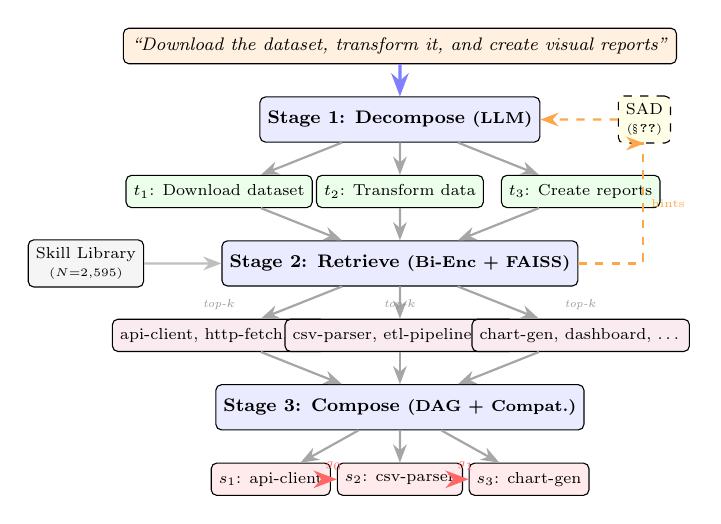
\begin{tikzpicture}[scale=0.82, every node/.append style={transform shape},
    >=Stealth, node distance=0.35cm and 0.5cm,
    stage/.style={draw, rounded corners=2pt, fill=blue!8, minimum height=0.7cm, minimum width=2.4cm, font=\footnotesize\bfseries, align=center},
    query/.style={draw, rounded corners=2pt, fill=orange!12, minimum height=0.55cm, font=\footnotesize, align=center},
    subtask/.style={draw, rounded corners=2pt, fill=green!8, minimum height=0.5cm, font=\scriptsize, align=center},
    skill/.style={draw, rounded corners=2pt, fill=purple!8, minimum height=0.5cm, font=\scriptsize, align=center},
    dag/.style={draw, rounded corners=2pt, fill=red!8, minimum height=0.5cm, font=\scriptsize, align=center},
    arrow/.style={->, thick, color=gray!70},
    bigarrow/.style={->, very thick, color=blue!50},
    lbl/.style={font=\tiny\itshape, color=gray!80},
]
\node[query, minimum width=6cm] (query) {\textit{``Download the dataset, transform it, and create visual reports''}};
\node[stage, below=0.5cm of query] (stage1) {Stage 1: Decompose {\scriptsize (LLM)}};
\draw[bigarrow] (query) -- (stage1);
\node[subtask, below=0.5cm of stage1, xshift=-2.8cm] (t1) {$t_1$: Download dataset};
\node[subtask, below=0.5cm of stage1] (t2) {$t_2$: Transform data};
\node[subtask, below=0.5cm of stage1, xshift=2.8cm] (t3) {$t_3$: Create reports};
\draw[arrow] (stage1) -- (t1); \draw[arrow] (stage1) -- (t2); \draw[arrow] (stage1) -- (t3);
\node[stage, below=0.5cm of t2] (stage2) {Stage 2: Retrieve {\scriptsize (Bi-Enc + FAISS)}};
\draw[arrow] (t1) -- (stage2); \draw[arrow] (t2) -- (stage2); \draw[arrow] (t3) -- (stage2);
\node[skill, below=0.5cm of stage2, xshift=-2.8cm] (c1) {api-client, http-fetch, \ldots};
\node[skill, below=0.5cm of stage2] (c2) {csv-parser, etl-pipeline, \ldots};
\node[skill, below=0.5cm of stage2, xshift=2.8cm] (c3) {chart-gen, dashboard, \ldots};
\draw[arrow] (stage2) -- (c1); \draw[arrow] (stage2) -- (c2); \draw[arrow] (stage2) -- (c3);
\node[lbl, above=0.02cm of c1] {top-$k$}; \node[lbl, above=0.02cm of c2] {top-$k$}; \node[lbl, above=0.02cm of c3] {top-$k$};
\node[stage, below=0.5cm of c2] (stage3) {Stage 3: Compose {\scriptsize (DAG + Compat.)}};
\draw[arrow] (c1) -- (stage3); \draw[arrow] (c2) -- (stage3); \draw[arrow] (c3) -- (stage3);
\node[dag, below=0.5cm of stage3, xshift=-2cm] (s1) {$s_1$: api-client};
\node[dag, below=0.5cm of stage3] (s2) {$s_2$: csv-parser};
\node[dag, below=0.5cm of stage3, xshift=2cm] (s3) {$s_3$: chart-gen};
\draw[arrow] (stage3) -- (s1); \draw[arrow] (stage3) -- (s2); \draw[arrow] (stage3) -- (s3);
\draw[->, very thick, color=red!60] (s1) -- node[above, font=\tiny] {$g_0$} (s2);
\draw[->, very thick, color=red!60] (s2) -- node[above, font=\tiny] {$g_1$} (s3);
\node[draw, dashed, rounded corners=2pt, fill=yellow!10, minimum height=0.5cm, font=\scriptsize, align=center, right=1.2cm of stage1] (sad) {SAD\\{\tiny (\S\ref{sec:sad})}};
\draw[->, dashed, thick, color=orange!70] (stage2.east) -- ++(1.0,0) |- node[right, pos=0.25, font=\tiny, color=orange!70] {hints} (sad.south);
\draw[->, dashed, thick, color=orange!70] (sad.west) -- (stage1.east);
\node[draw, rounded corners=2pt, fill=gray!8, font=\scriptsize, minimum height=0.4cm, align=center, left=1.2cm of stage2] (lib) {Skill Library\\{\tiny ($N{=}2{,}595$)}};
\draw[arrow, color=gray!50] (lib) -- (stage2);
\end{tikzpicture}
\caption{\system{} 系统概览。查询被分解为子任务，每个子任务通过双编码器检索匹配技能，最后组合为 DAG。虚线箭头：SAD 反馈环路（\S\ref{sec:sad}）。}
\label{fig:overview}
\end{figure*}

% ============================================================
\section{相关工作}
\label{sec:related}

\paragraph{工具选择与路由。}
LLM 的工具选择已通过 API 检索~\citep{patil2023gorilla,qin2023toolllm}、工具文档匹配~\citep{hao2024toolkengpt}和层级路由~\citep{xu2025skillrouter}等方式进行研究。
AnyTool~\citep{du2024anytool} 使用自反思机制导航层级 API 池，CRAFT~\citep{yuan2024craft} 通过检索为每个查询创建专门的工具集。
SkillRouter~\citep{xu2025skillrouter} 与我们的工作最为接近，引入了面向单技能路由的双编码器方法。
然而，上述方法均独立地为每个查询选择工具，未对组合式任务联合优化分解、检索和技能间兼容性。

\paragraph{工具增强的 LLM 基准。}
工具使用评估受到日益关注。
API-Bank~\citep{li2023apibank} 和 ToolQA~\citep{zhuang2024toolqa} 分别对单工具和多步工具使用进行基准测试。
ToolSandbox~\citep{lu2024toolsandbox} 提供有状态的评估框架，MetaTool~\citep{huang2024metatool} 关注\emph{是否}使用工具的决策。
TaskBench~\citep{shen2023taskbench} 评估多步任务，但基于固定工具集而非从大规模库中检索。
\benchmark{} 是首个专门针对数千技能之上\emph{组合式路由}的基准。

\paragraph{任务分解与规划。}
基于 LLM 的任务分解已通过提示策略~\citep{wei2022chain,zhou2022least,khot2023decomposed}、规划框架~\citep{huang2022language,wang2023plan}和智能体系统~\citep{yao2023react,shinn2023reflexion}进行探索。
\citet{press2023measuring} 识别了语言模型中的"组合性差距"，为基于分解的方法提供了动机。
TPTU~\citep{ruan2024tptu} 和 AgentFlan~\citep{chen2024agentflan} 研究联合任务规划与工具使用。
我们的贡献是一种新颖的\emph{技能感知}分解方法，分解器由技能库本身提供信息，形成检索增强的反馈环路。

\paragraph{检索增强生成。}
基于双编码器的稠密检索~\citep{karpukhin2020dense,ni2022sentence} 已广泛应用于知识密集型 NLP 任务。
我们将此范式适配于技能检索，并进一步扩展至为上游分解阶段提供信息——利用检索结果作为分解指引。

% ============================================================
\section{问题形式化}
\label{sec:problem}

\paragraph{技能库。}
技能库 $\mathcal{S} = \{s_1, \ldots, s_N\}$ 包含 $N$ 个技能。
每个技能 $s_i$ 是一个元组 $(n_i, d_i, b_i, C_i)$，其中 $n_i$ 为名称，$d_i$ 为自然语言描述，$b_i$ 为完整规范正文（指令、示例、配置），$C_i \subseteq \mathcal{C}$ 为功能分类体系 $\mathcal{C}$ 中的类别集合。

\paragraph{组合式技能路由。}
给定需要多种能力的复杂查询 $q$，目标是生成：
\begin{enumerate}[nosep,leftmargin=*]
  \item 分解 $D(q) = [t_1, \ldots, t_K]$，包含 $K$ 个原子子任务。
  \item 技能指派 $\sigma: [t_1, \ldots, t_K] \to \mathcal{S}^K$，将每个子任务映射到一个技能。
  \item 执行计划（DAG）$G = (V, E)$，指定步骤间的依赖关系。
\end{enumerate}

组合式路由函数为 $f: q \to (D, \sigma, G)$，优化：
\begin{equation}
\max_{D, \sigma, G} \sum_{k=1}^{K} \text{rel}(t_k, \sigma(t_k)) + (1\!-\!\alpha) \!\!\!\sum_{(i,j) \in E}\!\!\! \text{compat}(\sigma_i, \sigma_j)
\label{eq:routing}
\end{equation}
其中 $\text{rel}(\cdot)$ 度量子任务-技能相关性，$\text{compat}(\cdot)$ 度量技能间兼容性，$\alpha \in [0, 1]$ 控制相关性-兼容性权衡（在公式~\ref{eq:selection}~中实例化）。
联合优化公式~\ref{eq:routing}~通常是不可行的，我们的级联流水线（\S\ref{sec:method}）提供了一个可行的近似；SAD（\S\ref{sec:sad}）通过将检索信号反馈到分解阶段进一步缩小近似差距。

% ============================================================
\section{方法：\system{}}
\label{sec:method}

\system{} 通过三个级联阶段实现组合式技能路由（图~\ref{fig:overview}）。

\subsection{阶段一：任务分解}

给定复杂查询 $q$，任务分解器使用指令微调的 LLM 生成有序原子子任务列表：
\begin{equation}
D(q) = \text{LLM}(p_{\text{sys}}, p_{\text{user}}(q)) = [t_1, \ldots, t_K]
\end{equation}
其中 $p_{\text{sys}}$ 是指导模型将查询分解为子任务的系统提示，每个子任务恰好需要一项技能。
输出约束为 JSON 字符串数组以确保可靠解析。

我们应用模型原生的对话模板（如 Qwen 模型的 ChatML）以确保正确的指令遵循。
备用解析器处理 LLM 产生编号列表或其他非 JSON 格式的情况。

\subsection{阶段二：技能检索}

对于每个子任务 $t_k$，使用双编码器架构从技能库中检索 top-$m$ 个候选技能：
\begin{equation}
\text{cand}(t_k) = \text{top-}m_{s \in \mathcal{S}} \; \cos(E_q(t_k), E_s(s))
\end{equation}
其中 $E_q$ 和 $E_s$ 分别为查询编码器和技能编码器（共享参数），使用 BGE-large-en-v1.5~\citep{xiao2023bge} 实现。

\paragraph{技能表示。}
我们研究两种编码策略：
\begin{itemize}[nosep,leftmargin=*]
  \item \textbf{仅元数据}：$\text{repr}(s) = n_s \oplus d_s$（名称和描述）
  \item \textbf{包含正文}：$\text{repr}(s) = n_s \oplus d_s \oplus b_s[:L]$（含截断正文）
\end{itemize}
其中 $\oplus$ 表示拼接，$L=2000$ 字符。

嵌入向量经 $L_2$ 归一化后使用 FAISS~\citep{johnson2019faiss} 建立索引以实现高效内积搜索。

\subsection{阶段三：依赖感知的 DAG 规划}
\label{sec:compose}

不同于假设固定顺序执行的先前工作，\system{} 推断任务依赖并识别可并行化的子任务，生成\emph{有向无环图}（DAG）作为执行计划。

\paragraph{依赖检测。}
给定子任务 $[t_1, \ldots, t_K]$，使用三种互补信号检测成对依赖：
\begin{enumerate}[nosep,leftmargin=*]
  \item \textbf{I/O 类型重叠}：若 $t_i$ 的预期输出类型与 $t_j$ 的所需输入类型有交集，则推断 $t_i \to t_j$。
  \item \textbf{生产者-消费者模式}：精选关键词集识别输出产生动作（\emph{generate, fetch, extract}）和输入消费动作（\emph{parse, analyze, deploy}）。若 $t_i$ 匹配生产者模式且 $t_j$ 匹配消费者模式，则推断依赖。
  \item \textbf{语言标记}：$t_j$ 描述中出现"\emph{then}""、"\emph{after}""、"\emph{based on}"等短语表示对先前步骤的显式依赖。
\end{enumerate}
若未检测到依赖，规划器保守地退回到顺序链式执行。

\paragraph{并行组分配。}
给定依赖边 $E$，通过拓扑层级分配（Kahn 算法）为每个子任务分配并行组 $g(t_k)$：
\begin{equation}
g(t_k) = \begin{cases} 0 & \text{if } \text{indeg}(t_k) = 0 \\ \max_{(t_i, t_k) \in E}\; g(t_i) + 1 & \text{otherwise} \end{cases}
\label{eq:parallel}
\end{equation}
具有相同组编号的子任务无互相依赖，可并行执行，将关键路径长度从 $K$（完全顺序）缩短至 DAG 深度 $d \leq K$。

\paragraph{多维兼容性。}
我们定义上游技能 $s_a$ 与下游候选 $s_b$ 之间的四维兼容性函数：
\begin{equation}
\text{compat}(s_a, s_b) = \sum_{d \in \mathcal{D}} w_d \cdot \phi_d(s_a, s_b)
\label{eq:compat}
\end{equation}
其中 $\mathcal{D} = \{\text{io}, \text{cat}, \text{tag}, \text{kw}\}$：$\phi_\text{io}$ 通过类型强制转换矩阵度量 I/O 类型兼容性；$\phi_\text{cat}$ 和 $\phi_\text{tag}$ 在类别和标签上计算 Jaccard 相似度；$\phi_\text{kw}$ 检测生产者-消费者关键词共现。权重设置为 $(0.4, 0.2, 0.2, 0.2)$，基于 30 个查询的验证集网格搜索；结果对权重变化具有鲁棒性（$\pm$0.1 的变化使 $\catrecall$@1 变化 $<$0.5\%）。

\paragraph{DAG 感知的技能选择。}
最终每步技能结合检索相关性与 DAG 前驱兼容性：
\begin{equation}
\sigma(t_k) = \arg\max_{s \in \text{cand}(t_k)} \alpha \!\cdot\! \text{sim}(t_k, s) + (1\!-\!\alpha) \!\cdot\! \bar{c}_k(s)
\label{eq:selection}
\end{equation}
其中 $\bar{c}_k(s) = |\text{pred}(k)|^{-1}\!\sum_{i \in \text{pred}(k)} \text{compat}(\sigma_i, s)$ 对所有 DAG 前驱的兼容性取平均。

\subsection{技能感知分解（SAD）}
\label{sec:sad}

我们实验的一个关键洞察是：LLM 分解器产生的通用子任务描述与技能元数据对齐不佳。
我们提出\emph{技能感知分解}（SAD），一种检索增强反馈环路，使分解器获知可用技能。
给定初始分解 $D^{(0)}(q)$ 和阶段二的检索结果 $\text{cand}(t_k)$，SAD 构造提示集 $\mathcal{H}$，包含所有候选列表并集中的 top-$H$ 个技能名称。
分解器使用原始查询和 $\mathcal{H}$ 重新提示：
\begin{equation}
D^{(1)}(q) = \text{LLM}(p_{\text{sys}}, p_{\text{SAD}}(q, \mathcal{H}))
\end{equation}
其中 $p_{\text{SAD}}$ 将"可能相关的可用技能：$\mathcal{H}$"附加到分解提示中，使分解器能产生与实际技能名称更好对齐的子任务描述。
至关重要的是，即使第一轮分解质量较差，SAD 仍然有效：虽然不精确，但各子任务描述仍包含与任务相关的关键词，使检索器能浮现广泛相关的技能。由此产生的提示（hint）提供了用户查询语言与技能库命名约定之间的\emph{词汇桥梁}，使第二轮能生成与技能对齐的描述，而不依赖于第一轮的质量。
完整过程见算法~\ref{alg:sad}。

\begin{algorithm}[t]
\caption{技能感知分解（SAD）}
\label{alg:sad}
\small
\begin{algorithmic}[1]
\REQUIRE 查询 $q$，技能库 $\mathcal{S}$，检索器 $R$，提示数量 $H$
\ENSURE 精化后的分解 $D^{(1)}(q)$
\STATE \textbf{第一轮（原始）：} $D^{(0)}(q) = [t_1, \ldots, t_K] \gets \text{LLM}(p_{\text{sys}}, q)$
\FOR{$k = 1$ to $K$}
  \STATE $\text{cand}(t_k) \gets R.\text{retrieve}(t_k, \text{top\_k}{=}H)$
\ENDFOR
\STATE $\mathcal{H} \gets \text{top-}H\text{ skills from } \bigcup_k \text{cand}(t_k)$
\STATE \textbf{第二轮（技能感知）：} $D^{(1)}(q) \gets \text{LLM}(p_{\text{sys}}, p_{\text{SAD}}(q, \mathcal{H}))$
\RETURN $D^{(1)}(q)$
\end{algorithmic}
\end{algorithm}

% ============================================================
\section{基准测试：\benchmark{}}
\label{sec:benchmark}

\subsection{技能池构建}

我们从 212 个公开 GitHub 仓库中收集采用 SKILL.md 规范格式的技能~\citep{anthropic2025skills}。
原始收集得到 11{,}011 个技能。
我们应用以下筛选流程：

\begin{enumerate}[nosep,leftmargin=*]
  \item \textbf{去重}：合并同名技能，缩减至 7{,}681 个唯一技能。
  \item \textbf{质量过滤}：移除无描述或描述短于 10 字符的技能。
  \item \textbf{分类}：使用名称和描述字段上的关键词匹配，将技能分配到 17 个功能类别（表~\ref{tab:categories}）。反关键词防止误分类（如"debug"技能从"deployment"中排除）。未匹配任何类别或匹配多个冲突类别的技能被排除。
  \item 最终技能池包含 \textbf{2{,}595} 个已分类技能。
\end{enumerate}

\begin{table}[t]
\centering
\small
\setlength{\tabcolsep}{4pt}
\begin{tabular}{lrl}
\toprule
\textbf{类别} & \textbf{数量} & \textbf{示例} \\
\midrule
代码生成器 & 389 & prd-generator, nextjs-dev \\
API 客户端 & 312 & stripe-api, github-api \\
测试编写器 & 248 & unit-test-gen, qa-suite \\
数据处理器 & 221 & csv-parser, etl-pipeline \\
代码分析器 & 187 & code-review, lint-checker \\
文档编写器 & 176 & blog-writer, doc-gen \\
部署 & 142 & k8s-deploy, ci-cd-setup \\
安全 & 118 & vuln-scanner, audit-tool \\
可视化 & 97 & chart-gen, dashboard-builder \\
搜索 & 96 & web-search, code-search \\
\midrule
\multicolumn{2}{l}{\textit{+ 其余 7 个类别}} & 共 609 个 \\
\bottomrule
\end{tabular}
\caption{\benchmark{} 中前 10 个技能类别（共 17 个）。完整技能池包含来自 212 个仓库的 2{,}595 个技能。}
\label{tab:categories}
\end{table}

\subsection{查询生成}

组合式查询通过将不同类别的技能组合为多步任务来生成：

\paragraph{难度级别。}
\begin{itemize}[nosep,leftmargin=*]
  \item \textbf{简单}（117 个查询）：2 个技能，2 个类别
  \item \textbf{中等}（120 个查询）：3 个技能，3 个类别
  \item \textbf{困难}（63 个查询）：4--5 个技能，4--5 个类别
\end{itemize}

每个查询关联有真实子任务描述（源自实际技能描述）、真实技能 ID、所需类别和顺序执行序列。
基准共包含 300 个查询，涉及 523 个唯一的真实技能。

\paragraph{文本重叠披露。}
由于真实子任务描述源自技能元数据，子任务描述与技能库中的技能描述之间存在大量词汇重叠。
自动分析显示真实子任务与对应技能描述的平均 ROUGE-L 为 0.845，平均 BLEU-1 为 0.980，其中 37.8\% 为完全复制。
这解释了近乎完美的 oracle 检索性能（R@1 = 99.5\%），意味着模板查询上的绝对检索分数应被视为上界估计。
我们的人工撰写查询评估（\S\ref{sec:sad-results}）提供了互补评估，具有自然短语多样性，其中性能大幅下降（如 $\catrecall$@1：SAD 下 30.8\% vs 54.2\%），证实模板分数高估了真实性能。

\subsection{评估指标}

我们从三个粒度进行评估：

\paragraph{步骤级指标。}
\begin{itemize}[nosep,leftmargin=*]
  \item \textbf{技能召回率@$k$}（R@$k$）：真实技能出现在 top-$k$ 候选中的步骤比例。
  \item \textbf{类别召回率@$k$}（$\catrecall$@$k$）：\emph{正确类别中任何技能}出现在 top-$k$ 中的步骤比例。此宽松指标更具实用性，因为同一类别内的许多技能在功能上可互换。
\end{itemize}

\paragraph{链级指标。}
\begin{itemize}[nosep,leftmargin=*]
  \item \textbf{链精确匹配}（Chain$_E$）：\emph{所有}步骤均选择了精确真实技能的查询比例。
  \item \textbf{链类别匹配}（$\chaincat$）：每个查询中选择了正确类别技能的步骤平均比例。
\end{itemize}

\paragraph{分解准确率（DA）。}预测子任务数与真实值匹配的查询比例。
DA 是严格的结构指标；一个有 3 个真实步骤的查询被分解为 4 个（包含一个额外有效中间步骤）将得到 DA=0。我们主要使用 DA 诊断分解粒度；$\catrecall$@1 是主要质量指标。

% ============================================================
\section{实验设置}
\label{sec:setup}

\paragraph{LLM 分解器。}
我们比较五个开源指令微调模型，跨三个规模：
Qwen2.5-7B-Instruct、Qwen2.5-14B-Instruct 和 Qwen2.5-72B-Instruct~\citep{qwen2.5}，
Llama-3.1-8B-Instruct~\citep{dubey2024llama3}，以及
Mistral-7B-Instruct-v0.3~\citep{jiang2023mistral}。
生成使用温度 $\tau=0.1$，$\text{top}_p=0.9$，最大生成 256 个 token。
我们通过三次不同随机种子运行验证低方差：vanilla 和 SAD 配置下 $\catrecall$@1 标准差均 $\leq$0.003。

\paragraph{检索器。}
BGE-large-en-v1.5~\citep{xiao2023bge}（1024 维）作为双编码器，使用 FAISS IndexFlatIP 进行精确内积搜索。
除非另有说明，检索时设 $k=10$。

\paragraph{基线方法。}
\begin{itemize}[nosep,leftmargin=*]
  \item \textbf{单技能}（Single-Skill）：不进行分解；使用完整查询检索一组技能并应用于所有步骤。代表当前的单技能路由方法。
  \item \textbf{LLM 直接选择}（LLM-Direct）：不进行分解；向 LLM 提供查询和 top-50 检索技能的描述，直接选择使用哪些技能。测试上下文内选择能否替代显式分解。
  \item \textbf{Oracle 分解}：使用真实子任务描述进行检索，建立分解质量的上界。
\end{itemize}

\paragraph{硬件。}
7--14B 模型在单张 NVIDIA A100-80GB GPU 上运行。
72B 模型使用四张 A100-80GB GPU，通过 \texttt{device\_map="auto"} 自动张量并行。

% ============================================================
\section{实验结果}
\label{sec:results}

\subsection{主要结果}

表~\ref{tab:main} 展示了所有配置下的主要实验结果。

\begin{table*}[t]
\centering
\small
\resizebox{\textwidth}{!}{
\begin{tabular}{llccccccc}
\toprule
\textbf{方法} & \textbf{信号} & \textbf{DA} & \textbf{R@1} & \textbf{R@10} & $\catrecall$\textbf{@1} & $\catrecall$\textbf{@10} & \textbf{Chain}$_E$ & $\chaincat$ \\
\midrule
\multicolumn{9}{l}{\textit{基线方法}} \\
单技能 & Meta & -- & 0.000 & 0.029 & 0.211 & 0.698 & 0.000 & 0.216 \\
单技能 & Body & -- & 0.002 & 0.028 & 0.285 & 0.633 & 0.000 & 0.293 \\
Oracle 分解 & Meta & 1.000 & \textbf{0.995} & \textbf{1.000} & \textbf{1.000} & \textbf{1.000} & \textbf{0.987} & \textbf{1.000} \\
Oracle 分解 & Body & 1.000 & 0.990 & 1.000 & 0.998 & 1.000 & 0.970 & 0.998 \\
\midrule
\multicolumn{9}{l}{\textit{完整流水线（\system{}）}} \\
Qwen2.5-7B & Meta & 0.360 & 0.005 & 0.034 & 0.339 & 0.649 & 0.000 & 0.316 \\
Qwen2.5-7B & Body & 0.370 & 0.008 & 0.029 & \underline{0.363} & \underline{0.662} & 0.000 & \underline{0.345} \\
Llama-3.1-8B & Meta & 0.000 & 0.002 & 0.016 & 0.216 & 0.507 & 0.000 & 0.210 \\
Mistral-7B & Meta & 0.177 & 0.005 & 0.036 & 0.243 & 0.607 & 0.000 & 0.248 \\
\midrule
\multicolumn{9}{l}{\textit{+ 技能感知分解（\S\ref{sec:sad-results}）}} \\
Qwen2.5-7B + SAD & Meta & \underline{0.690} & \underline{0.012} & \underline{0.068} & \underline{0.542} & \underline{0.753} & \underline{0.003} & \underline{0.521} \\
\bottomrule
\end{tabular}
}
\caption{在 \benchmark{} 上的主要结果。\textbf{粗体}：总体最优。\underline{下划线}：完整流水线中最优。R@$k$：技能召回率@$k$。$\catrecall$@$k$：类别召回率@$k$。Chain$_E$：链精确匹配。$\chaincat$：链类别匹配。DA：分解准确率。}
\label{tab:main}
\end{table*}

\paragraph{分解是瓶颈。}
Oracle 分解达到 R@1 = 99.5\% 和完美的类别准确率。
最优 LLM 分解器（Qwen2.5-7B）仅达 $\catrecall$@1 = 36.3\%，证实分解质量是主要瓶颈。

\paragraph{组合式路由优于单技能。}
我们的完整流水线达到 $\catrecall$@1 = 33.9\%，显著优于单技能基线（21.1\%），验证了即使近似分解也有助于组合式路由。

\paragraph{元数据与正文表现相当。}
仅元数据检索达到 oracle R@1 = 99.5\% vs 正文感知的 99.0\%。
在完整流水线中，正文感知略有优势（$\catrecall$@1：36.3\% vs 33.9\%），但编码成本更高，说明简洁的元数据已捕获关键辨别信号。

\subsection{分解器比较}

\begin{table}[t]
\centering
\small
\begin{tabular}{lccc}
\toprule
\textbf{分解器} & \textbf{DA} & $\catrecall$\textbf{@1} & $\chaincat$ \\
\midrule
Qwen2.5-7B & \textbf{0.360} & \textbf{0.339} & \textbf{0.316} \\
Mistral-7B & 0.177 & 0.243 & 0.248 \\
Llama-3.1-8B & 0.000 & 0.216 & 0.210 \\
\midrule
Oracle & 1.000 & 1.000 & 1.000 \\
\bottomrule
\end{tabular}
\caption{分解器比较（均使用仅元数据检索）。Qwen2.5-7B 达到最优的分解准确率和下游路由性能。}
\label{tab:decomposer}
\end{table}

表~\ref{tab:decomposer} 比较了三个 LLM 分解器。
Qwen2.5-7B 显著优于其他模型，分解准确率达 36.0\%，而 Mistral 为 17.7\%，Llama 为 0\%。

\paragraph{过度分解是主要失败模式。}
分解模式分析（图~\ref{fig:decomp_dist}）揭示 Llama-3.1-8B 系统性地过度分解：中位输出为 9 个子任务，而真实分布在 2--3 处达峰。
Llama 无单个分解匹配真实数量，解释了其 0\% 的分解准确率。
Mistral 呈现类似但程度较轻的趋势，Qwen 的分布与真实值最为接近。

\subsection{难度分析}

\begin{table}[t]
\centering
\small
\begin{tabular}{llccc}
\toprule
\textbf{方法} & \textbf{难度} & $\catrecall$\textbf{@1} & $\catrecall$\textbf{@10} \\
\midrule
\multirow{3}{*}{单技能} & 简单 & 0.201 & 0.774 \\
& 中等 & 0.267 & 0.667 \\
& 困难 & 0.146 & 0.675 \\
\midrule
\multirow{3}{*}{Qwen + Meta} & 简单 & 0.214 & 0.637 \\
& 中等 & 0.367 & 0.658 \\
& 困难 & \textbf{0.410} & 0.646 \\
\midrule
\multirow{3}{*}{Qwen + Body} & 简单 & 0.252 & 0.607 \\
& 中等 & \textbf{0.403} & \textbf{0.728} \\
& 困难 & 0.407 & 0.623 \\
\bottomrule
\end{tabular}
\caption{按难度级别的性能分析。基于分解的路由在更难查询上展现更大优势。}
\label{tab:difficulty}
\end{table}

表~\ref{tab:difficulty} 按难度级别分解结果。
基于分解的流水线在\emph{较难查询上优势最大}：对于困难查询（4--5 个技能），Qwen + Meta 达到 $\catrecall$@1 = 41.0\%，而单技能基线为 14.6\%（+181\%）。
这一模式表明，随着任务复杂度增加，分解变得越来越重要。

\subsection{技能感知分解结果}
\label{sec:sad-results}

\paragraph{SAD 消融实验。}

\begin{table}[t]
\centering
\small
\begin{tabular}{lccc}
\toprule
\textbf{提示数 $H$} & \textbf{DA} & $\catrecall$\textbf{@1} & $\chaincat$ \\
\midrule
0（原始） & 0.360 & 0.339 & 0.316 \\
5 & 0.457 & 0.468 & 0.445 \\
10 & 0.537 & 0.519 & 0.498 \\
15 & 0.690 & \textbf{0.542} & \textbf{0.521} \\
25 & \textbf{0.790} & 0.474 & 0.451 \\
\bottomrule
\end{tabular}
\caption{SAD 消融实验（Qwen2.5-7B）。DA 单调递增，但 $\catrecall$@1 在 $H{=}15$ 处达峰，揭示了噪声-对齐权衡。}
\label{tab:sad-ablation}
\end{table}

表~\ref{tab:sad-ablation} 展示了提示数量 $H$ 的消融结果。
DA 单调递增（36.0\% 至 79.0\%），但 $\catrecall$@1 在 $H{=}15$ 达峰（54.2\%），随后在 $H{=}25$ 时下降（47.4\%），揭示了噪声-对齐权衡。
从 $H{=}0$ 到 $H{=}5$ 的不成比例跳跃（+38\% $\catrecall$@1）表明，即使少量提示也能从根本上将分解器从自由形式转向技能感知生成，额外提示的边际收益递减。

\paragraph{跨模型泛化。}

\begin{table}[t]
\centering
\small
\begin{tabular}{llccc}
\toprule
\textbf{模型} & \textbf{模式} & \textbf{DA} & $\catrecall$\textbf{@1} & $\chaincat$ \\
\midrule
\multirow{2}{*}{Qwen2.5-7B} & 原始 & 0.360 & 0.339 & 0.316 \\
 & +SAD & 0.690 & \textbf{0.542} & \textbf{0.521} \\
\midrule
\multirow{2}{*}{Qwen2.5-14B} & 原始 & 0.280 & 0.297 & 0.280 \\
 & +SAD & 0.443 & 0.385 & 0.377 \\
\midrule
\multirow{2}{*}{Llama-3.1-8B} & 原始 & 0.000 & 0.216 & 0.210 \\
 & +SAD & 0.217 & 0.339 & 0.323 \\
\midrule
\multirow{2}{*}{Mistral-7B} & 原始 & 0.177 & 0.242 & 0.248 \\
 & +SAD & 0.273 & 0.307 & 0.301 \\
\midrule
\multirow{2}{*}{Qwen2.5-72B} & 原始 & 0.627 & 0.368 & 0.358 \\
 & +SAD & 0.503 & 0.483 & \underline{0.518} \\
\bottomrule
\end{tabular}
\caption{跨模型 SAD 结果（$H{=}15$）。SAD 在五个模型（7--72B）上均提升了路由性能。\textbf{粗体}：最优。\underline{下划线}：次优。7B+SAD 超越了 10 倍规模的 72B 原始模型。}
\label{tab:sad-crossmodel}
\end{table}

表~\ref{tab:sad-crossmodel} 显示 SAD 在不同模型家族中具有泛化性，$\catrecall$@1 提升从 +26.9\%（Mistral）到 +59.9\%（Qwen-7B）。
所有模型均使用 $H{=}15$ 以确保公平比较；针对各模型单独调参可能取得更好结果。
\textbf{Qwen2.5-7B+SAD（54.2\%）优于 72B 原始模型（36.8\%）}，表明检索增强分解可超越 10 倍规模的模型。
72B 模型的 SAD 将 DA 从 62.7\% 降至 50.3\%，同时 $\catrecall$@1 提升至 48.3\%。
我们将此 DA 下降归因于\emph{提示诱导合并}：72B 模型本身具备细粒度分解能力（原始平均 2.7 个子任务），当技能提示暗示更粗粒度时会合并子任务，产生更少但与技能更对齐的描述。
分析证实 72B+SAD 平均每查询 2.3 个子任务（vs 原始 2.7），且保留的子任务与技能元数据的词汇重叠更高（平均 ROUGE-L 0.72 vs 0.58）。
我们推测 72B 的 $\catrecall$@1 低于 7B+SAD 反映了\emph{提示锚定}效应：较大模型倾向于逐字复制技能名称而非将提示用作词汇指引，当复制的名称与真实技能不完全匹配时降低了检索对齐——这一模式在 14B 异常中也有观察（附录~\ref{app:14b}）。
14B 异常（性能低于 7B）源于过度分解和较低的 JSON 解析率；详见附录~\ref{app:14b}。

\paragraph{人工撰写查询泛化。}
为补充模板评估，三名计算机科学研究生独立撰写了 55 个组合式查询（22 简单、23 中等、10 困难），遵循要求自然措辞且无法访问技能名称或描述的指引。
SAD 将 $\catrecall$@1 从 18.8\% 提升至 30.8\%（+63.8\%）。
困难查询下降（17.0\% $\to$ 9.4\%）：我们将此归因于\emph{提示稀释}——困难查询需要 4--5 个跨多种类别的技能，因此 $H{=}15$ 的提示集不可避免地包含许多无关技能，误导了分解。
此外，困难人工查询使用更间接的表述（如"搭建完整的 CI/CD 工作流"），加剧了难度。
较低的绝对数值证实人工措辞多样性仍具挑战性。

\subsection{消融实验：约束分解}

为分离分解\emph{粒度}（步骤数）与分解\emph{质量}（子任务描述）的影响，我们进行消融实验：将 LLM 分解截断或填充以匹配真实步骤数。

约束分解达到 $\catrecall$@1 = 33.9\%，与非约束流水线相同。
这表明主要挑战不在于预测步骤\emph{数量}，而在于生成与目标技能\emph{语义对齐}的子任务描述。
即使步骤数正确，LLM 生成的子任务描述可能过于通用或使用与技能元数据不同的术语，导致检索失配。

\subsection{上下文窗口分析}
\label{sec:context}

表~\ref{tab:context} 量化了上下文节省：暴露所有 2{,}595 个技能消耗约 1.04M token，超过大多数 LLM 上下文限制；\system{} 将每查询减少至 2--5 个技能（$>$99\% 缩减）。

\begin{table}[t]
\centering
\small
\begin{tabular}{lrrr}
\toprule
\textbf{策略} & \textbf{工具数} & \textbf{估计 Token} & \textbf{缩减比例} \\
\midrule
所有工具（朴素） & 2{,}595 & $\sim$1{,}038K & --- \\
Top-$k$ 平面检索 & 10 & $\sim$4{,}000 & 99.6\% \\
\system{}（平均链） & 2.9 & $\sim$1{,}160 & 99.9\% \\
\bottomrule
\end{tabular}
\caption{上下文窗口消耗（$\sim$400 token/工具）。组合式路由将消耗减少两个数量级。}
\label{tab:context}
\end{table}

% ============================================================
\section{分析}
\label{sec:analysis}

我们检查了 Qwen + Meta 流水线的 50 个失败案例：
\textbf{过度分解}（36\%）、\textbf{通用描述}（28\%）、\textbf{词汇不匹配}（22\%）和\textbf{不足分解}（14\%）。
Oracle R@1（99.5\%）证实检索器质量；0.5\% 的失败出现在技能具有近乎相同元数据的情况下。

% ============================================================
\section{讨论}
\label{sec:discussion}

\paragraph{分解差距。}
Oracle 分解实现近乎完美的检索，但最优 LLM 分解器（Qwen-7B）仅达 $\catrecall$@1 = 33.9\%；扩展至 72B 也仅达 36.8\%。
SAD 缩小了这一差距：\textbf{7B+SAD（54.2\%）超越 72B 原始模型 7.4 个百分点}，使用 $10\times$ 少的参数，跨模型结果确认 SAD 具有模型无关性。

\paragraph{分解 vs 直接选择。}
一种替代方案是让 LLM 从 top-50 检索技能描述中直接选择。
表~\ref{tab:llm-direct} 比较了此方法与我们的流水线。

\begin{table}[t]
\centering
\small
\begin{tabular}{llcc}
\toprule
\textbf{模型} & \textbf{方法} & $\catrecall$\textbf{@1} & $\chaincat$ \\
\midrule
\multirow{3}{*}{Qwen2.5-7B} & 原始流水线 & 0.339 & 0.316 \\
 & LLM 直接选择 & 0.396 & --- \\
 & +SAD 流水线 & \textbf{0.542} & \textbf{0.521} \\
\midrule
\multirow{3}{*}{Qwen2.5-72B} & 原始流水线 & 0.368 & 0.358 \\
 & LLM 直接选择 & 0.470 & --- \\
 & +SAD 流水线 & 0.483 & 0.518 \\
\bottomrule
\end{tabular}
\caption{分解 vs 直接选择。LLM 直接选择给模型提供 top-50 技能描述进行上下文内选择。\textbf{7B+SAD 优于 72B LLM 直接选择}，尽管参数少 $10\times$。}
\label{tab:llm-direct}
\end{table}

72B LLM 直接选择达到 $\catrecall$@1 = 47.0\%，但\textbf{7B+SAD（54.2\%）仍超越之}，确认结构化分解配合检索反馈优于暴力上下文内选择。

\paragraph{元数据 vs 正文。}
仅元数据检索与正文感知编码表现相当，说明组合式分解产生的目标查询自然地与简洁元数据对齐。

\paragraph{可扩展性。}
FAISS 检索可扩展至数千技能（中位延迟 568ms，p95: 1.26s）。
DAG 规划达到 80.0\% 边检测率和 53.7\% 功能一致性（附录~\ref{app:dag-pilot}）；组合式路由将上下文减少超过 99\%（\S\ref{sec:context}）。

% ============================================================
\section{结论}
\label{sec:conclusion}

我们形式化了组合式技能路由并提出 \system{}，一个分解-检索-组合框架，其中 SAD 在五个模型（7--72B）上将 $\catrecall$@1 提升 60\%——配合 SAD 的 7B 模型优于不使用 SAD 的 72B 模型。
在 \benchmark{} 上，oracle 检索近乎完美，确认分解是瓶颈。代码、数据和 \benchmark{} 将在论文接收后公开。

% ============================================================
% 参考文献
\bibliography{references}

% ============================================================
\section*{局限性}

我们的基准使用模板生成查询，文本重叠较高（ROUGE-L=0.845）；虽然 55 个人工撰写查询在简单/中等难度上显示一致的 SAD 增益，但困难查询（4--5 个技能）性能下降。
DAG 规划器的并行化能力缺乏偏序真实值评估。
我们的评估聚焦检索；完整端到端评估（实际技能执行）和基于学习的依赖预测仍为未来工作。
SAD 需要两轮 LLM 推理，分解延迟约增加一倍（7B 模型在 A100 上共约 1.6 秒）。
我们仅评估开源模型；闭源模型可能实现更高的原始分解质量，但 SAD 是正交方法，可进一步提升其性能。
我们假设子任务与技能之间为一对一映射；放宽为多对多映射是未来工作。
困难子集（63 个模板查询、10 个人工查询）统计效力有限；在困难人工查询上观察到的 SAD 下降可能部分反映采样噪声。

\section*{伦理声明}

本工作仅使用公开可用的开源技能仓库，不涉及人类受试者或个人数据。
我们鼓励在人工监督下负责任地部署技能路由系统。

% ============================================================
\appendix

\section{类别分类体系}
\label{app:categories}

\benchmark{} 中的 17 个功能类别为：
code\_generator、api\_client、test\_writer、data\_processor、code\_analyzer、writer、deployment、security、visualizer、search、refactorer、file\_converter、translator、database、monitoring、designer、git\_workflow。

\section{分解分布}
\label{app:decomp}

图~\ref{fig:decomp_dist} 展示了各 LLM 分解器预测的子任务数量分布与真实值的比较。

\begin{figure}[h]
\centering
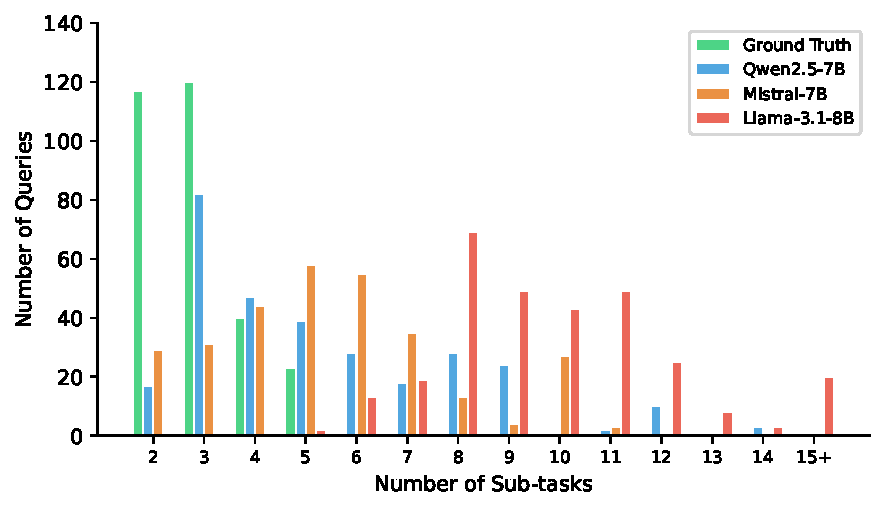
\includegraphics[width=\columnwidth]{figures/decomp_dist.pdf}
\caption{各分解器预测的子任务数量分布。Llama-3.1-8B 系统性地过度分解（中位 9 个子任务），而 Qwen2.5-7B 与真实分布最为接近（峰值在 2--3）。}
\label{fig:decomp_dist}
\end{figure}

\section{Top-$k$ 敏感性}
\label{app:topk}

使用 oracle 分解，R@1 = 99.5\% 在 $k=1$ 时即可达到，R@$k$ 在 $k=3$ 时达到 100\%，表明检索器具有很高的精确度。

\section{14B 异常分析}
\label{app:14b}

Qwen2.5-14B 表现低于 7B 变体的反直觉结果值得进一步检验。
分解模式分析揭示两个成因。
首先，14B 原始模型平均每查询产生 5.3 个子任务（vs 7B 的 2.9），42.7\% 的查询生成超过 5 个子任务——严重的过度分解碎片化了检索信号。
其次，14B 原始输出仅 71.3\% 可解析为有效 JSON（vs 7B 的 89.3\%），表明该规模下对结构化输出格式的遵循较弱。
使用 SAD 后，14B 的 JSON 解析率提升至 85.0\%，但 44.7\% 的查询退化为单子任务回退，表明模型逐字复制技能名称而非产生真正的分解。
这些发现表明更大的模型并不一定在结构化分解方面表现更好。

\section{DAG 规划器试验评估}
\label{app:dag-pilot}

表~\ref{tab:dag-pilot} 报告了在 20 个查询的分层试验集（8 简单、8 中等、4 困难）上使用 Qwen2.5-7B + SAD（$H{=}15$）的 DAG 规划器评估结果。

\begin{table}[h]
\centering
\small
\begin{tabular}{lcccccc}
\toprule
\textbf{难度} & \textbf{$n$} & \textbf{步骤准确率} & \textbf{边/查询} & \textbf{一致性} & \textbf{延迟 (ms)} \\
\midrule
简单 & 8 & 0.75 & 0.8 & 0.56 & 849 \\
中等 & 8 & 0.75 & 1.6 & 0.56 & 564 \\
困难 & 4 & 0.50 & 2.5 & 0.44 & 889 \\
\midrule
总计 & 20 & 0.70 & 1.4 & 0.54 & 743 \\
\bottomrule
\end{tabular}
\caption{DAG 规划器试验评估。步骤准确率：预测步骤数与真实值匹配的查询比例。边/查询：每查询检测到的平均依赖边数。一致性：功能一致性（相邻技能对具有兼容 I/O 类别的比例）。80\% 的查询至少检测到一条依赖边。中位延迟 568ms（p95: 1,261ms）。不同难度间的延迟变化反映小样本量（$n$=4--8）而非系统性趋势。}
\label{tab:dag-pilot}
\end{table}

\section{SAD 提示模板}
\label{app:sad-prompts}

\paragraph{系统提示（原始和 SAD 共用）。}
\begin{quote}
\small\ttfamily
You are a task decomposition assistant. Given a complex user query, break it down into atomic sub-tasks, each requiring exactly one tool or skill. Output a JSON array of strings. Each string should be a concise, actionable sub-task description.
\end{quote}

\paragraph{原始用户提示。}
\begin{quote}
\small\ttfamily
Decompose the following query into atomic sub-tasks:\\ \{query\}
\end{quote}

\paragraph{SAD 用户提示（第二轮）。}
\begin{quote}
\small\ttfamily
Decompose the following query into atomic sub-tasks.\\ Available skills that may be relevant: \{hint\_list\}\\ Query: \{query\}
\end{quote}

\noindent 其中 \texttt{\{hint\_list\}} 是第一轮检索到的 top-$H$ 个技能名称的逗号分隔列表（见算法~\ref{alg:sad}）。

\end{document}
